% !TeX program = pdflatex
\documentclass[10pt,aspectratio=169]{beamer}

% Metropolis theme
\usetheme[progressbar=frametitle,numbering=fraction]{metropolis}

\usepackage{amsmath,amssymb}
\usepackage{booktabs}
\usepackage{graphicx}
\usepackage{xcolor}
\usepackage{hyperref}
% --- put once in your preamble (optional, but nice) ---
\newcommand{\fin}[1]{\textcolor{blue}{\texttt{#1}}}
\newcommand{\eng}[1]{\textcolor{black}{\texttt{#1}}}
% ------------------------------------------------------------
% Finnish -> English naming (used throughout this file)
% ASIAKAS      -> CUSTOMER
% LASKU        -> INVOICE
% TUOTE        -> PRODUCT
% LASKU_RIVI   -> INVOICE_LINE
%
% astun        -> customer_id
% asnimi       -> customer_name
% kaup         -> city
% tyyppi       -> customer_type
% mpiiri       -> district
% laskuno      -> invoice_id
% vuosi        -> year
% lask_summa   -> invoice_total
% tila         -> status
% tuotetun     -> product_id
% tuotennimi   -> product_name
% malli        -> model
% ahinta       -> unit_price
% vari         -> color
% maara        -> quantity
% ------------------------------------------------------------

% Put these in your preamble (once)
\usetikzlibrary{matrix,arrows.meta,positioning,calc}

% helper rows for the table boxes
\newcommand{\trow}[2]{\texttt{#1}\hfill\texttt{\textbf{#2}}}
\newcommand{\trowpk}[2]{\underline{\texttt{#1}}\hfill\texttt{\textbf{#2}}}

\tikzset{
  rel/table/.style={
    matrix of nodes,
    nodes={
      draw,
      text width=30mm,
      minimum height=5.4mm,
      align=left,
      font=\tiny,
      inner xsep=2pt,
      inner ysep=1.2pt
    },
    row 1/.style={nodes={fill=black, text=white, font=\bfseries\small, align=center}},
    row 2/.style={nodes={fill=black!10}},
    row 3/.style={nodes={fill=black!2}},
    row 4/.style={nodes={fill=black!10}},
    row 5/.style={nodes={fill=black!2}},
    row 6/.style={nodes={fill=black!10}},
  },
  rel/fk/.style={thick, -{Latex[length=2.2mm]}}
}

% --- SQL highlighting ---
\newcommand{\sqlk}[1]{\textcolor{blue}{#1}}

\usepackage{listings}
\definecolor{dkgreen}{rgb}{0,0.6,0}
\definecolor{gray}{rgb}{0.5,0.5,0.5}
\definecolor{mauve}{rgb}{0.58,0,0.82}

\lstdefinestyle{sqlite}{
  language=SQL,
  morekeywords={TEXT,REAL,ROUND,CHAR,VARCHAR,INT,INTEGER,PRAGMA},
  basicstyle={\small\ttfamily},
  keywordstyle=\color{blue},
  commentstyle=\color{dkgreen},
  stringstyle=\color{mauve},
  numbers=none,
  showstringspaces=false,
  breaklines=true,
  breakatwhitespace=true,
  columns=flexible,
  tabsize=3,
  frame=single,
  rulecolor=\color{gray},
  xleftmargin=0.0em,
  framexleftmargin=0.0em,
   framexrightmargin=-1em,
  frameround=tttt,
}
\lstnewenvironment{codesql}{\lstset{style=sqlite}}{}

% Convenience
\newcommand{\partslide}[2]{%
  \begin{frame}[plain]
    \vfill
    {\Huge\textbf{#1}}\\[0.6em]
    {\Large #2}
    \vfill
  \end{frame}
}

\title{Database Programming in SQL -- Part I/II}
\subtitle{Introduction to SQL (2\,$\times$\,45 min)}
\author{Michael Emmerich}
\date{\today}

\begin{document}

\maketitle

\begin{frame}{Roadmap}
\begin{columns}[T,onlytextwidth]
\column{0.48\textwidth}
\textbf{Part I (45 min)}
\begin{itemize}
  \item What is SQL? (declarative)
  \item SQL vs. relational model
  \item Basic statement rules
  \item Querying one table: \sqlk{SELECT} / \sqlk{FROM} / \sqlk{WHERE}
  \item Sorting and limiting results
  \item \sqlk{NULL} basics
\end{itemize}
\column{0.52\textwidth}
\textbf{Part II (45 min)}
\begin{itemize}
  \item Querying multiple tables (joins)
  \item \sqlk{IN} and \sqlk{EXISTS} subqueries
  \item Explicit \sqlk{JOIN} syntax
  \item Set operations: \sqlk{UNION}
  \item Aggregation: \sqlk{SUM}, \sqlk{COUNT}, \sqlk{MIN/MAX/AVG}
  \item Grouping and \sqlk{HAVING}
\end{itemize}
\end{columns}
\end{frame}

% ----------------------- Part I -----------------------
\partslide{Part I}{SQL basics \& single-table queries}

\begin{frame}[fragile]{What is SQL?}
\begin{itemize}
  \item SQL (Structured Query Language) is a standardized language for interacting with relational databases.
  \item \textbf{Declarative}: you describe \emph{what} you want; the DBMS decides \emph{how} to compute it.
\end{itemize}
\vspace{0.7em}
\begin{codesql}
SELECT *
FROM table;
\end{codesql}
\end{frame}

\begin{frame}[fragile]{SQL vs. imperative code (intuition)}
\begin{columns}[T,onlytextwidth]
\column{0.4\textwidth}
\textbf{SQL (declarative)}
\begin{codesql}
SELECT *
FROM table;
\end{codesql}
\column{0.6\textwidth}
\textbf{Imperative (e.g., C\#)}
\begin{lstlisting}[language={[Sharp]C},basicstyle=\small\ttfamily]
for (int i = 0; i < table.Length; i++) {
  System.Console.WriteLine(table[i]);
}
\end{lstlisting}
\end{columns}
\vspace{0.6em}
\small In SQL, the optimizer can change the evaluation strategy without changing the result.
\end{frame}

\begin{frame}{Relational model \& SQL terminology}
\begin{center}
\begin{tabular}{ll}
\toprule
\textbf{Relational model} & \textbf{SQL}\\
\midrule
Relation & Table\\
Attribute & Column\\
Tuple & Row\\
\bottomrule
\end{tabular}
\end{center}
\vspace{0.8em}
\begin{itemize}
  \item SQL is often called \emph{relationally complete}: relational algebra operations (e.g., cartesian product, set union, join and others) can be expressed in SQL.
  \item Practical note: unless constrained (e.g., by a \sqlk{PRIMARY KEY}), tables may contain duplicate rows.
\end{itemize}
\end{frame}

\begin{frame}{SQL dialects \& sublanguages}
\begin{itemize}
  \item Different DBMSs implement (parts of) the standard with small differences: \textbf{SQL dialects}.
  \item Four common sublanguages:
  \begin{itemize}
    \item \textbf{DML} (Data Manipulation Language): \sqlk{SELECT}, \sqlk{INSERT}, \sqlk{UPDATE}, \sqlk{DELETE}
    \item \textbf{DDL} (Data Definition Language): \sqlk{CREATE}, \sqlk{ALTER}, \sqlk{DROP}
    \item \textbf{DCL} (Data Control Language): \sqlk{GRANT}, \sqlk{REVOKE}
    \item \textbf{TxCL} (Transaction Control): \sqlk{BEGIN}, \sqlk{COMMIT}, \sqlk{ROLLBACK}
  \end{itemize}
\end{itemize}
\end{frame}

\begin{frame}{SQL statements: basic rules}
\begin{itemize}
  \item Line breaks do not matter.
  \item Statements typically end with a semicolon \texttt{;}
  \item Keywords are case-insensitive: \texttt{SELECT} = \texttt{select}
  \item Identifier rules (typical): letters, digits, underscores; no spaces; do not start with a digit.
  \item Avoid using reserved keywords as table/column names.
\end{itemize}
\end{frame}

% ------------------------------------------------------------
% Single slide: left (0.4) text + right (0.6) diagram (EN names)
% ------------------------------------------------------------
\begin{frame}{CUSTOMER--INVOICE--PRODUCT: schema + foreign keys + table representation}

\begin{columns}[T,onlytextwidth]
\column{0.4\textwidth}
{\tiny
\setlength{\parskip}{0pt}
\setlength{\itemsep}{1pt}

\begin{block}{Relations (PK underlined)}
\begin{itemize}
  \item \texttt{CUSTOMER(}\underline{\texttt{customer\_id}}\texttt{, customer\_name, city, customer\_type, district)}
  \item \texttt{INVOICE(}\underline{\texttt{invoice\_id}}\texttt{, year, invoice\_total, status, customer\_id)}
  \item \texttt{PRODUCT(}\underline{\texttt{product\_id}}\texttt{, product\_name, model, unit\_price, color)}
  \item \texttt{INVOICE\_LINE(}\underline{\texttt{invoice\_id}}\texttt{, }\underline{\texttt{product\_id}}\texttt{, quantity)}
\end{itemize}
\end{block}

\vspace{-1mm}
\begin{block}{Foreign keys}
\begin{itemize}
  \item \texttt{INVOICE.customer\_id} $\rightarrow$ \texttt{CUSTOMER.customer\_id}
  \item \texttt{INVOICE\_LINE.invoice\_id} $\rightarrow$ \texttt{INVOICE.invoice\_id}
  \item \texttt{INVOICE\_LINE.product\_id} $\rightarrow$ \texttt{PRODUCT.product\_id}
\end{itemize}
\end{block}

\vspace{-1mm}
\begin{block}{Meaning (very short)}
\begin{itemize}
  \item A customer has invoices; each invoice has line items; each line item references a product.
\end{itemize}
\end{block}
}

\column{0.6\textwidth}
\centering

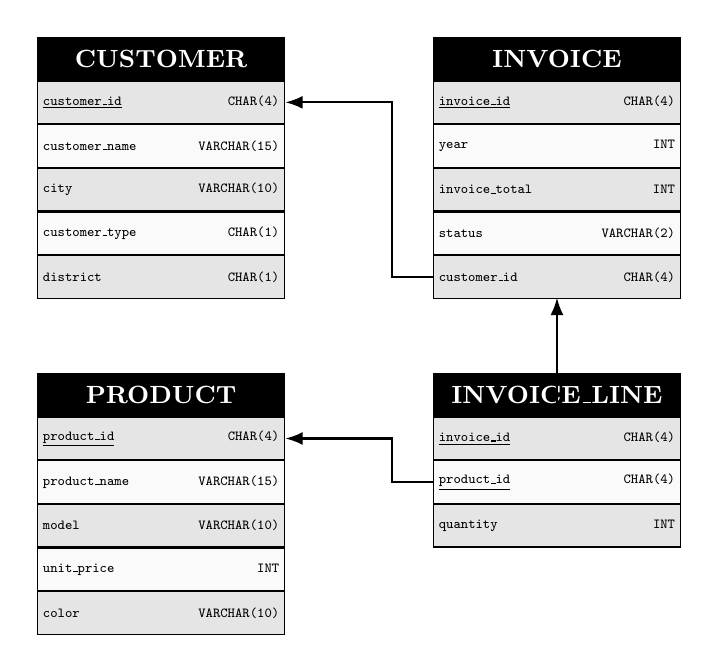
\begin{tikzpicture}[scale=0.58, transform shape]

\matrix (cust) [rel/table] {
  CUSTOMER\\
  \trowpk{customer\_id}{CHAR(4)}\\
  \trow{customer\_name}{VARCHAR(15)}\\
  \trow{city}{VARCHAR(10)}\\
  \trow{customer\_type}{CHAR(1)}\\
  \trow{district}{CHAR(1)}\\
};

\matrix (inv) [rel/table, right=28mm of cust.north east, anchor=north west] {
  INVOICE\\
  \trowpk{invoice\_id}{CHAR(4)}\\
  \trow{year}{INT}\\
  \trow{invoice\_total}{INT}\\
  \trow{status}{VARCHAR(2)}\\
  \trow{customer\_id}{CHAR(4)}\\
};

\matrix (prod) [rel/table, below=12mm of cust.south west, anchor=north west] {
  PRODUCT\\
  \trowpk{product\_id}{CHAR(4)}\\
  \trow{product\_name}{VARCHAR(15)}\\
  \trow{model}{VARCHAR(10)}\\
  \trow{unit\_price}{INT}\\
  \trow{color}{VARCHAR(10)}\\
};

\matrix (line) [rel/table, below=12mm of inv.south west, anchor=north west] {
  INVOICE\_LINE\\
  \trowpk{invoice\_id}{CHAR(4)}\\
  \trowpk{product\_id}{CHAR(4)}\\
  \trow{quantity}{INT}\\
};

% --- FK arrows
\draw[rel/fk] (inv-6-1.west) -- ++(-9mm,0) |- (cust-2-1.east);
\draw[rel/fk] (line-2-1.north) -- ++(0,0.6mm) -|
  ($ (inv-2-1.south) + (0mm,-38mm) $);
\draw[rel/fk] (line-3-1.west) -- ++(-9mm,0) |- (prod-2-1.east);

\end{tikzpicture}

\end{columns}
\end{frame}

% ------------------------------------------------------------
% Slide: Finnish -> English glossary (two columns)
% Place this right after the CUSTOMER--INVOICE--PRODUCT example slide.
% ------------------------------------------------------------
\begin{frame}{Running example: Finnish names (blue) and English names (black)}
\small
\begin{columns}[T,onlytextwidth]

\column{0.60\textwidth}

\begin{block}{We use a small sales database:}

\textbf{customers} have \textbf{invoices}; each invoice consists of \textbf{invoice lines}; each line references one \textbf{product}.\\
In the rest of the lecture, we use the \textbf{English} names consistently.
\end{block}

\vspace{5mm}
\begin{block}{Attributes grouped by table}
\scriptsize
\begin{tabular}{@{}l l@{}}
\toprule
\textbf{Table} & \textbf{Attributes (Finnish / English)}\\
\midrule
\fin{ASIAKAS} &
\fin{astun}\,/\eng{customer\_id},\;
\fin{asnimi}\,/\eng{customer\_name},\;
\fin{kaup}\,/\eng{city},\;
\fin{tyyppi}\,/\eng{customer\_type},\;
\fin{mpiiri}\,/\eng{district}\\
\addlinespace
\fin{LASKU} &
\fin{laskuno}\,/\eng{invoice\_id},\;
\fin{vuosi}\,/\eng{year},\;
\fin{lask\_summa}\,/\eng{invoice\_total},\;
\fin{tila}\,/\eng{status},\;
\fin{astun}\,/\eng{customer\_id}\\
\addlinespace
\fin{TUOTE} &
\fin{tuotetun}\,/\eng{product\_id},\;
\fin{tuotennimi}\,/\eng{product\_name},\;
\fin{malli}\,/\eng{model},\;
\fin{ahinta}\,/\eng{unit\_price},\;
\fin{vari}\,/\eng{color}\\
\addlinespace
\fin{LASKU\_RIVI} &
\fin{laskuno}\,/\eng{invoice\_id},\;
\fin{tuotetun}\,/\eng{product\_id},\;
\fin{maara}\,/\eng{quantity}\\
\bottomrule
\end{tabular}
\end{block}

\vspace{1mm}
\begin{block}{Foreign keys (arrows only here)}
\scriptsize
\eng{INVOICE.customer\_id} $\rightarrow$ \eng{CUSTOMER.customer\_id}\\
\eng{INVOICE\_LINE.invoice\_id} $\rightarrow$ \eng{INVOICE.invoice\_id}\\
\eng{INVOICE\_LINE.product\_id} $\rightarrow$ \eng{PRODUCT.product\_id}
\end{block}

\column{0.40\textwidth}

\begin{block}{Table (relation) names}
\footnotesize
\begin{tabular}{@{}ll@{}}
\toprule
\textbf{Finnish} & \textbf{English}\\
\midrule
\fin{ASIAKAS} & \eng{CUSTOMER}\\
\fin{LASKU} & \eng{INVOICE}\\
\fin{TUOTE} & \eng{PRODUCT}\\
\fin{LASKU\_RIVI} & \eng{INVOICE\_LINE}\\
\bottomrule
\end{tabular}
\end{block}

\end{columns}
\end{frame}





% ------------------------------------------------------------
% Added: DDL vs. DML + CREATE TABLE examples (SQLite)
% Placed here to bridge the running schema to the upcoming query examples.
% ------------------------------------------------------------

\begin{frame}[fragile]{SQL building blocks: DDL vs.\ DML (SQLite)}
\small
\begin{itemize}
  \item We start from a \textbf{relational schema} (structure) and then write SQL.
  \item \textbf{DDL (Data Definition Language)} defines the \emph{structure}:
        tables, attributes, primary keys, foreign keys, constraints.
  \item \textbf{DML (Data Manipulation Language)} changes the \emph{data inside} tables:
        inserting, updating, deleting tuples.
\end{itemize}

\vspace{1mm}
\begin{block}{Running example schema (lecture notation)}
\footnotesize
\texttt{CUSTOMER(}\underline{\texttt{customer\_id}}\texttt{, customer\_name, city, customer\_type, district)}\\
\texttt{INVOICE(}\underline{\texttt{invoice\_id}}\texttt{, year, invoice\_total, status, customer\_id)}\\
\texttt{PRODUCT(}\underline{\texttt{product\_id}}\texttt{, product\_name, model, unit\_price, color)}\\
\texttt{INVOICE\_LINE(}\underline{\texttt{invoice\_id}}\texttt{, }\underline{\texttt{product\_id}}\texttt{, quantity)}\\{\scriptsize (relationship table)}\\
\end{block}

\vspace{-1mm}
\textbf{Typical commands}
\begin{codesql}
-- DDL: define structure
CREATE TABLE ... ;
-- DML: insert data (tuples)
INSERT INTO ... VALUES ... ;
\end{codesql}
\end{frame}

% -----------------------------
\begin{frame}[fragile]{DDL in SQLite: \texttt{CREATE TABLE} and primary keys}
\small
\begin{itemize}
  \item \sqlk{PRIMARY KEY} enforces \textbf{uniqueness} and (in SQLite) implies \textbf{NOT NULL} for the key columns.
  \item In this running example: \texttt{customer\_id} identifies a customer, \texttt{product\_id} identifies a product.
\end{itemize}

\vspace{1mm}
\begin{block}{DDL example: base tables}
\end{block}
\begin{lstlisting}[style=sqlite,basicstyle=\footnotesize\ttfamily]
CREATE TABLE CUSTOMER(
  customer_id   CHAR(4)      PRIMARY KEY,
  customer_name VARCHAR(15)  NOT NULL,
  city          VARCHAR(10),
  customer_type CHAR(1),
  district      CHAR(1)
);
CREATE TABLE PRODUCT(
  product_id    CHAR(4)      PRIMARY KEY,
  product_name  VARCHAR(15)  NOT NULL,
  model         VARCHAR(10),
  unit_price    INT          NOT NULL,
  color         VARCHAR(10)
);
\end{lstlisting}
\end{frame}

% -----------------------------
\begin{frame}[fragile]{Foreign keys + inserts: \texttt{INVOICE\_LINE} (SQLite)}
\small
\begin{itemize}
  \item \textbf{Foreign keys (FK)} enforce \textbf{referential integrity}:
        e.g., \texttt{INVOICE.customer\_id} must exist in \texttt{CUSTOMER(customer\_id)}.
  \item Composite PK \texttt{(invoice\_id, product\_id)} prevents product appearing twice in the same invoice.
\end{itemize}
\vspace{1mm}

\begin{lstlisting}[style=sqlite,basicstyle=\scriptsize\ttfamily]
PRAGMA foreign_keys = ON;
CREATE TABLE INVOICE_LINE(
  invoice_id   CHAR(4),
  product_id   CHAR(4),
  quantity     INT,
  PRIMARY KEY (invoice_id, product_id),
  FOREIGN KEY (invoice_id) REFERENCES INVOICE(invoice_id),
  FOREIGN KEY (product_id) REFERENCES PRODUCT(product_id)
);
INSERT INTO CUSTOMER(customer_id, customer_name, city, customer_type, district)
VALUES ('C001', 'Ada', 'Jyvaskyla', 'A', '1');
INSERT INTO PRODUCT(product_id, product_name, model, unit_price, color)
VALUES ('P010', 'Database Book', '2nd', 45, 'Blue');
INSERT INTO INVOICE(invoice_id, year, invoice_total, status, customer_id)
VALUES ('I100', 2026, 45, 'OK', 'C001');
INSERT INTO INVOICE_LINE(invoice_id, product_id, quantity)
VALUES ('I100', 'P010', 1);
\end{lstlisting}
\vspace{1mm}
\footnotesize More DDL elements (constraints, \sqlk{ALTER}, \sqlk{DROP}, indexes) are covered later in the course.
\end{frame}

\begin{frame}[fragile]{General form of a query (one table)}
\begin{codesql}
SELECT column1, column2, ...
FROM   table;
\end{codesql}
\vspace{0.8em}
\begin{itemize}
  \item \sqlk{SELECT}: which columns (projection)
  \item \sqlk{FROM}: which table(s)
\end{itemize}
\end{frame}

\begin{frame}[fragile]{Selecting columns vs. selecting all}
\begin{columns}[T,onlytextwidth]
\column{0.52\textwidth}
\textbf{Pick specific columns}
\begin{codesql}
SELECT customer_id, customer_name, city, customer_type, district
FROM   customer;
\end{codesql}
\column{0.48\textwidth}
\textbf{Pick all columns}
\begin{codesql}
SELECT *
FROM   customer;
\end{codesql}
\end{columns}
\vspace{0.6em}
\small Prefer explicit column lists in real applications (clarity, stability, performance).
\end{frame}

\begin{frame}[fragile]{Filtering rows with \sqlk{WHERE}}
\begin{codesql}
SELECT *
FROM   product
WHERE  unit_price > 100
  AND  unit_price < 2000;
\end{codesql}
\vspace{0.6em}
\begin{itemize}
  \item Comparison operators: \texttt{=}, \texttt{<}, \texttt{<=}, \texttt{>}, \texttt{>=}, \texttt{<>} (or \texttt{!=})
  \item Combine conditions with \sqlk{AND}, \sqlk{OR}, and \sqlk{NOT}
\end{itemize}
\end{frame}

\begin{frame}[fragile]{Operator precedence \& parentheses}
\begin{itemize}
  \item Like arithmetic, parentheses control evaluation order.
  \item In many SQL dialects, \sqlk{AND} binds tighter than \sqlk{OR}.
  \item When in doubt: add parentheses.
\end{itemize}
\vspace{0.6em}
\begin{codesql}
SELECT product_id, product_name, unit_price
FROM   product
WHERE (product_name LIKE 't%' OR product_name LIKE 's%')
  AND (unit_price > 200 OR unit_price < 20);
\end{codesql}
\end{frame}

\begin{frame}[fragile]{Strings and pattern matching with \sqlk{LIKE}}
Wildcards (common):
\begin{itemize}
  \item \texttt{\%} matches any sequence of characters (including empty)
  \item \texttt{\_} matches exactly one character
\end{itemize}
\vspace{0.6em}
\begin{codesql}
-- Names starting with K, or ending in 'Ltd'
SELECT customer_name, district, customer_type
FROM   customer
WHERE  customer_name LIKE 'K%'
   OR  customer_name LIKE '%Ltd';
\end{codesql}
\end{frame}

\begin{frame}[fragile]{Other handy predicates: \sqlk{IN} and \sqlk{BETWEEN}}
\begin{columns}[T,onlytextwidth]
\column{0.52\textwidth}
\textbf{Membership}
\begin{codesql}
SELECT *
FROM   customer
WHERE  district IN ('I', 'L');
\end{codesql}
\column{0.48\textwidth}
\textbf{Range (inclusive)}
\begin{codesql}
SELECT *
FROM   product
WHERE  unit_price BETWEEN 100 AND 1000;
\end{codesql}
\end{columns}
\end{frame}

\begin{frame}[fragile]{\sqlk{NULL} values (missing/unknown)}
\begin{itemize}
  \item \sqlk{NULL} represents ``no value'' (unknown, missing, not applicable).
  \item Comparing with \sqlk{NULL} using \texttt{=} does \emph{not} work as you might expect.
  \item Use \sqlk{IS NULL} / \sqlk{IS NOT NULL}.
\end{itemize}
\vspace{0.6em}
\begin{codesql}
SELECT *
FROM   product
WHERE  unit_price IS NULL;
\end{codesql}
\end{frame}

\begin{frame}[fragile]{Ordering and limiting results}
\begin{columns}[T,onlytextwidth]
\column{0.55\textwidth}
\textbf{Order by one or more columns}
\begin{codesql}
SELECT customer_id, customer_type, district
FROM   customer
WHERE  customer_name <> 'Kajo'
ORDER BY customer_type, customer_name;
\end{codesql}
\column{0.45\textwidth}
\textbf{Limit output size}
\begin{codesql}
SELECT invoice_id, year, status
FROM   invoice
ORDER BY year DESC
LIMIT  1;
\end{codesql}
\end{columns}
\end{frame}

\begin{frame}[plain]
\vfill
\centering
{\Large \textbf{End of Part I}}\\[0.8em]
\small Next: multi-table queries, joins, set operations, aggregation.
\vfill
\end{frame}

% ----------------------- Part II -----------------------
\partslide{Part II}{Multi-table queries, joins \& aggregation}

\begin{frame}{Why multiple tables?}
\begin{itemize}
  \item Real databases split information across tables (normalization, clarity, integrity).
  \item Queries often need to combine rows from multiple tables based on a \textbf{join condition}.
  \item SQL offers several equivalent ways to express joins.
\end{itemize}
\end{frame}

\begin{frame}{Join idea (conceptually)}
\begin{itemize}
  \item A join condition matches related rows (often via key/foreign key).
  \item Typical pattern: \texttt{table1.key = table2.foreign\_key}
  \item The DBMS chooses an efficient algorithm (nested-loop, hash join, sort-merge, \dots).
\end{itemize}
\end{frame}

\begin{frame}[fragile]{Joining via a subquery: \sqlk{IN}}
\begin{codesql}
-- Products that have been billed at least once
SELECT product_name
FROM   product
WHERE  product_id IN (
  SELECT product_id
  FROM   invoice_line
);
\end{codesql}
\end{frame}

\begin{frame}[fragile]{Joining via a correlated subquery: \sqlk{EXISTS}}
\begin{codesql}
SELECT p.product_name
FROM   product p
WHERE  EXISTS (
  SELECT *
  FROM   invoice_line il
  WHERE  p.product_id = il.product_id
);
\end{codesql}
\vspace{0.4em}
\small \sqlk{EXISTS} returns true if the subquery finds at least one matching row.
\end{frame}

\begin{frame}[fragile]{Joining with comparison operators (classic style)}
\begin{codesql}
SELECT DISTINCT p.product_name
FROM   product p, invoice_line il
WHERE  p.product_id = il.product_id;
\end{codesql}
\vspace{0.4em}
\begin{itemize}
  \item Works, but can become hard to read for many tables.
  \item Use \sqlk{DISTINCT} if duplicates can appear.
\end{itemize}
\end{frame}

\begin{frame}[fragile]{Explicit \sqlk{JOIN} syntax (recommended)}
\begin{codesql}
SELECT DISTINCT p.product_name
FROM   product p
JOIN   invoice_line il
       ON p.product_id = il.product_id;
\end{codesql}
\vspace{0.6em}
\small SQL also defines other join types (e.g., \sqlk{LEFT OUTER JOIN}); we focus on inner joins here.
\end{frame}

\begin{frame}[fragile]{Set operations: \sqlk{UNION}}
\begin{itemize}
  \item Combine results of multiple queries into one result table.
  \item The queries must return the same number of columns (compatible types).
\end{itemize}
\vspace{0.6em}
\begin{codesql}
SELECT model AS models_and_product_names
FROM   product
UNION
SELECT product_name
FROM   product;
\end{codesql}
\end{frame}

\begin{frame}[fragile]{Aggregate functions (analytics)}
\begin{itemize}
  \item Aggregates compute one value from many rows.
  \item Common aggregates: \sqlk{SUM}, \sqlk{COUNT}, \sqlk{MIN}, \sqlk{MAX}, \sqlk{AVG}
\end{itemize}
\vspace{0.6em}
\begin{codesql}
-- Sum of unit prices
SELECT SUM(unit_price) AS total_unit_price
FROM   product;
\end{codesql}
\end{frame}

\begin{frame}[fragile]{Counting rows and distinct values}
\begin{columns}[T,onlytextwidth]
\column{0.52\textwidth}
\textbf{Count rows}
\begin{codesql}
SELECT COUNT(*) AS customer_count
FROM   customer;
\end{codesql}
\column{0.48\textwidth}
\textbf{Count distinct values}
\begin{codesql}
SELECT COUNT(DISTINCT city) AS city_count
FROM   customer;
\end{codesql}
\end{columns}
\end{frame}

\begin{frame}[fragile]{\sqlk{MIN}, \sqlk{MAX}, \sqlk{AVG}}
\begin{columns}[T,onlytextwidth]
\column{0.5\textwidth}
\begin{codesql}
SELECT MAX(unit_price) - MIN(unit_price) AS price_range
FROM   product;
\end{codesql}
\column{0.5\textwidth}
\begin{codesql}
SELECT AVG(unit_price) AS avg_unit_price
FROM   product;
\end{codesql}
\end{columns}
\end{frame}

\begin{frame}[fragile]{Grouping with \sqlk{GROUP BY}}
\begin{itemize}
  \item Group rows by one (or more) columns, then aggregate per group.
\end{itemize}
\vspace{0.6em}
\begin{codesql}
-- Sum of unit prices by color
SELECT SUM(unit_price) AS total_price, color
FROM   product
GROUP BY color;
\end{codesql}
\end{frame}

\begin{frame}[fragile]{Filtering groups with \sqlk{HAVING}}
\begin{itemize}
  \item \sqlk{WHERE} filters rows \emph{before} grouping.
  \item \sqlk{HAVING} filters groups \emph{after} grouping.
\end{itemize}
\vspace{0.6em}
\begin{codesql}
SELECT COUNT(DISTINCT p.product_id) AS product_count, p.color
FROM   product p, invoice_line il
WHERE  p.product_id = il.product_id
GROUP BY p.color
HAVING product_count > 2
ORDER BY product_count DESC;
\end{codesql}
\end{frame}

% -----------------------------
\begin{frame}[fragile]{Example: \sqlk{GROUP BY} (average grade per subject)}
\small
\begin{columns}[T,onlytextwidth]
% -------- LEFT COLUMN --------
\column{0.48\textwidth}

\begin{block}{Table: \texttt{Enrolled}}
\footnotesize
\centering
\begin{tabular}{@{}lll@{}}
\toprule
\textbf{Name} & \textbf{Subject} & \textbf{Grade}\\
\midrule
Anna   & Topology  & 4\\
Bernd  & Music     & 5\\
Corina & Music     & 4\\
Donald  & Topology  & 1\\
Emmi   & Databases & 5\\
\bottomrule
\end{tabular}
\end{block}

\vspace{1mm}
\begin{block}{SQL query}
\begin{codesql}
SELECT Subject, AVG(Grade) AS avgGrade
FROM Enrolled
WHERE Name <> 'Emmi'
GROUP BY Subject;
\end{codesql}
\end{block}

% -------- RIGHT COLUMN --------
\column{0.52\textwidth}

\begin{block}{After \sqlk{WHERE} (rows removed before grouping)}
\footnotesize
\centering
\begin{tabular}{@{}lll@{}}
\toprule
\textbf{Name} & \textbf{Subject} & \textbf{Grade}\\
\midrule
Anna   & Topology & 4\\
Donald  & Topology & 1\\
Bernd  & Music    & 5\\
Corina & Music    & 4\\
\bottomrule
\end{tabular}
\end{block}

\vspace{1mm}
\begin{block}{Result after \sqlk{GROUP BY}}
\footnotesize
\centering
\begin{tabular}{@{}lr@{}}
\toprule
\textbf{Subject} & \textbf{AvgGrade}\\
\midrule
Topology & 2.5\\
Music    & 4.5\\
\bottomrule
\end{tabular}
\end{block}

\end{columns}
\end{frame}

% -----------------------------
\begin{frame}[fragile]{Example: \sqlk{HAVING} (filter groups after aggregation)}
\small
\begin{itemize}
  \item \sqlk{WHERE} filters \textbf{rows before} grouping.
  \item \sqlk{HAVING} filters \textbf{groups after} \sqlk{GROUP BY} (often using aggregates like \sqlk{AVG}, \sqlk{COUNT}).
\end{itemize}

\vspace{1mm}
\begin{columns}[T,onlytextwidth]
\column{0.55\textwidth}
\begin{block}{SQL query with \sqlk{HAVING}}
\begin{codesql}
SELECT Subject, AVG(Grade) AS avgGrade
FROM Enrolled
WHERE Name <> 'Emmi'
GROUP BY Subject
HAVING AVG(Grade) >= 3;
\end{codesql}
\end{block}

\column{0.45\textwidth}
\begin{block}{Groups and averages (from previous slide)}
\footnotesize
\centering
\begin{tabular}{@{}lr@{}}
\toprule
\textbf{Subject} & \textbf{AvgGrade}\\
\midrule
Topology & 2.5\\
Music    & 4.5\\
\bottomrule
\end{tabular}
\end{block}

\vspace{1mm}
\begin{block}{After \sqlk{HAVING} (keep only avgGrade $>=$ 3)}
\footnotesize
\centering
\begin{tabular}{@{}lr@{}}
\toprule
\textbf{Subject} & \textbf{AvgGrade}\\
\midrule
Music & 4.5\\
\bottomrule
\end{tabular}
\end{block}

\end{columns}
\end{frame}



\begin{frame}[fragile]{(Optional) Finding ``missing'' matches: \sqlk{NOT IN} / \sqlk{NOT EXISTS}}
\begin{itemize}
  \item Useful pattern: find rows in one table that have \emph{no related row} in another table.
\end{itemize}
\vspace{0.6em}
\begin{codesql}
-- Customers who have never been billed in year 2011
SELECT customer_id, customer_name
FROM   customer
WHERE  customer_id NOT IN (
  SELECT customer_id
  FROM   invoice
  WHERE  year = 2011
);
\end{codesql}
\end{frame}

\begin{frame}{Summary}
\begin{itemize}
  \item Single-table queries: \sqlk{SELECT} / \sqlk{FROM} / \sqlk{WHERE} + \sqlk{ORDER BY} + \sqlk{LIMIT}
  \item Be careful with \sqlk{NULL}: use \sqlk{IS NULL} / \sqlk{IS NOT NULL}
  \item Multi-table queries: joins via \sqlk{IN}, \sqlk{EXISTS}, comparisons, or explicit \sqlk{JOIN}
  \item Set operation: \sqlk{UNION}
  \item Aggregation: \sqlk{SUM}, \sqlk{COUNT}, \sqlk{MIN/MAX/AVG} with \sqlk{GROUP BY} and \sqlk{HAVING}
\end{itemize}
\end{frame}

\begin{frame}[plain]
\vfill
\centering
{\Large \textbf{Next up in the course}}\\[0.8em]
\begin{itemize}
  \item Data definition (tables, keys, constraints)
  \item Updates and transactions
  \item Views and access control
\end{itemize}
\vfill
\end{frame}

\end{document}
